\documentclass[11pt]{article}
\usepackage{graphicx} % Required for inserting images
\usepackage{hyperref}
\usepackage{listings}
\usepackage{caption}
\usepackage{minted}
\usepackage{todonotes}
\usepackage[a4paper, total={6in, 8in},margin=1in,top=0.81in,bottom=1.25in]{geometry}
\usepackage{fancyhdr}
\usepackage{pdfpages}
\usepackage{sectsty}
\usepackage{fontspec}
\usepackage{multicol}

\setmainfont{Carlito}
\sectionfont{\fontsize{24}{30}\selectfont}  % 24pt size, 30pt line spacing
\subsectionfont{\fontsize{18}{24}\selectfont}
\subsubsectionfont{\fontsize{14}{18}\selectfont}
\renewcommand{\listingscaption}{Izvorni kod}
\renewcommand{\listoflistingscaption}{Spisak izvornih kodova}
\pagestyle{fancy}
\fancyhf{}
\fancyfoot[L]{\fontsize{11}{13}\selectfont Aleksa Bajat, Intermedijarne reprezentacije izvornog koda u prednjem kraju (frontend-u) rustc kompajlera}
\fancyfoot[R]{\newline\fontsize{11}{13}\selectfont \thepage}

\title{Intermedijarne reprezentacije izvornog koda u prednjem kraju (frontend-u) rustc kompajlera}
\author{Aleksa Bajat}
\date{September 2024}

\begin{document}
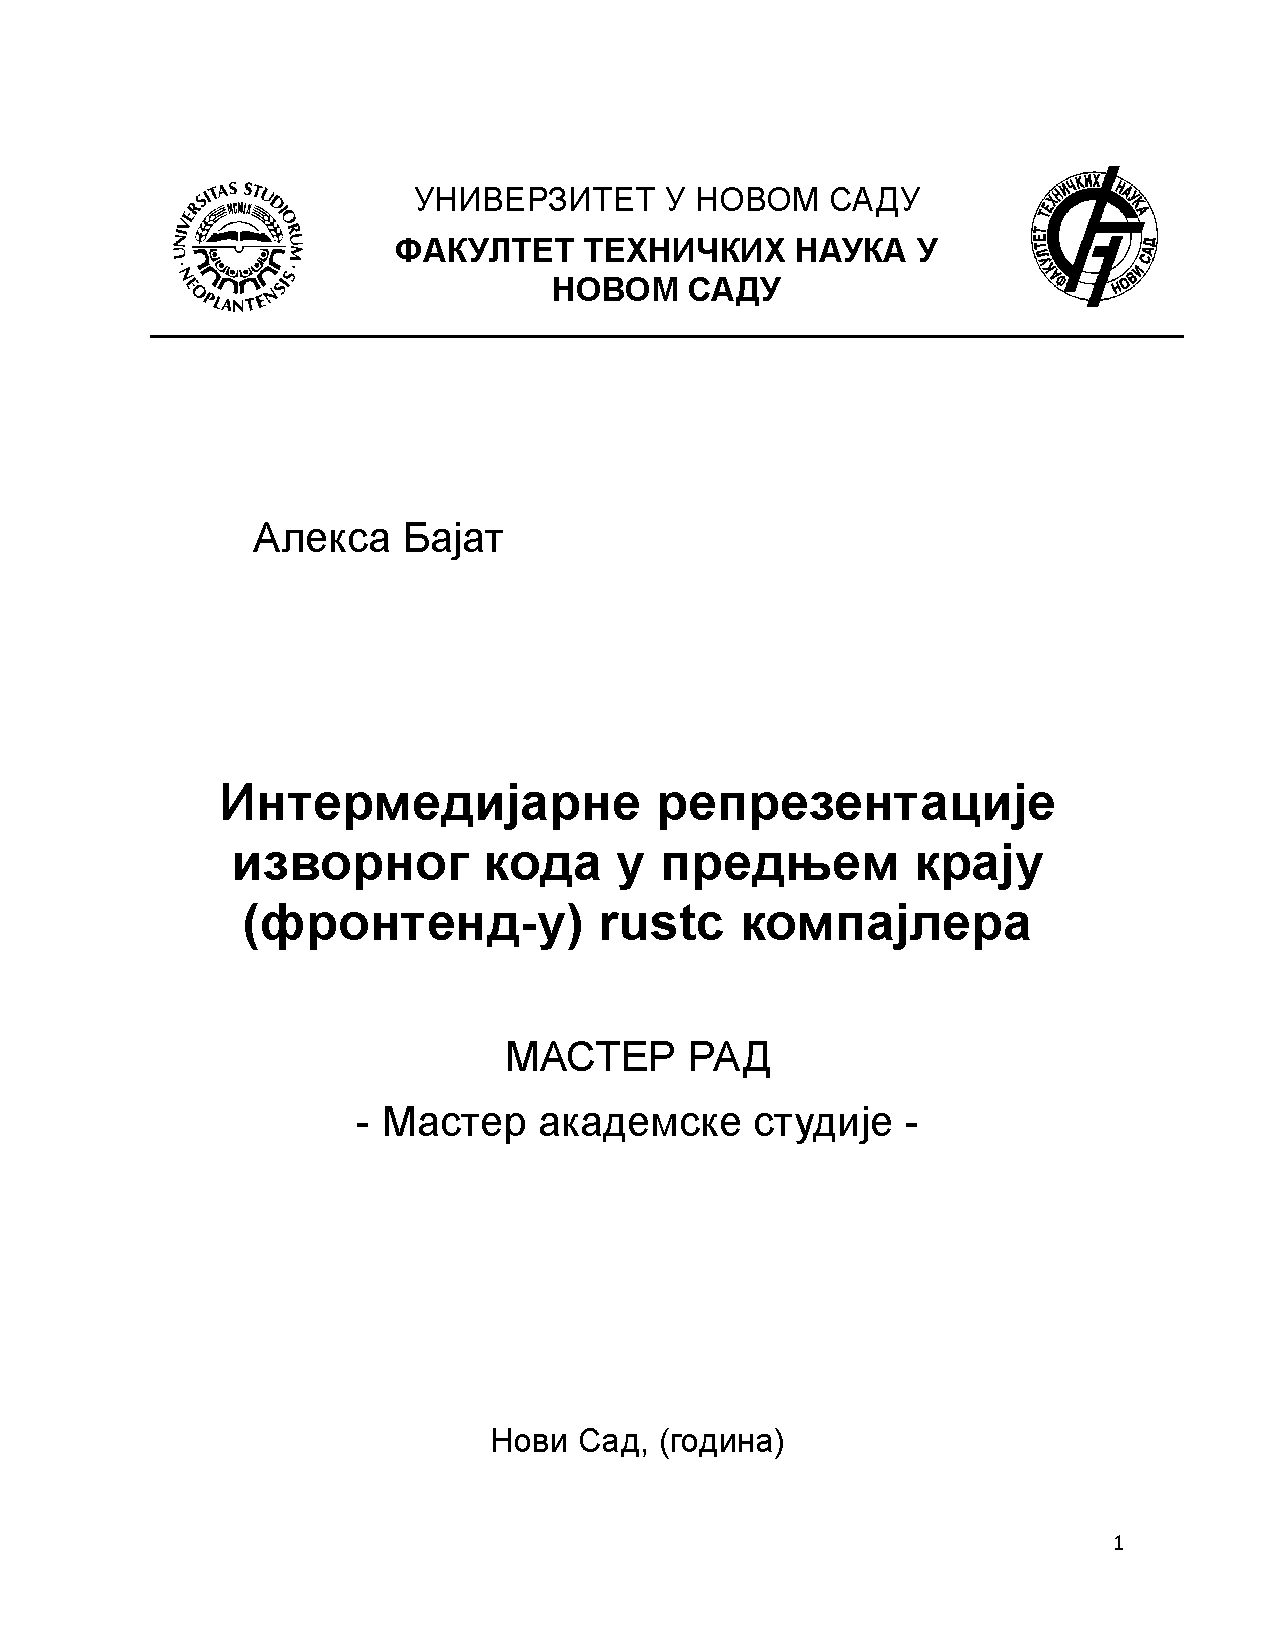
\includepdf[pages={1-6}]{MscTemplate.pdf}
\newpage
\section{Spisak skraćenica}
\newpage
\tableofcontents
\newpage

\section{Uvod}

U svetu razvoja sistema visokih performansi, operativnih sistema, drajvera i bilo kog drugog kritičnog softvera koriste se jezici niskog nivoa kao što su C i C++.
Tokom godina Microsoft je uvideo da je preko 70\% bezbednosnih slabosti nastalo pogrešnom manipulacijom i korupcijom memorije [1]. 
C nema odbrambene mehanizme od ovakvih problema (pored potencijalnih dodatnih upozorenja koja se mogu ostvariti dvostrukom upotrebom GCC i Clang kompajlera), dok C++ uprkos dodavanju konstrukta kao što su \verb|unique_ptr|, \verb|shared_ptr| i \verb|weak_ptr| interoperabilnost sa starijim standardima ili bibliotekama zahteva korišćenje sirovih pokazivača. 

Rust jezik je nastao sa ciljem da reši ovaj problem. Podrazumevana upotreba jezika je inherentno bezbedna sa aspekta memorije i paralelizma. Bezbednost se ostvaruje robustnim sistemom tipova, novog načina rukovanja memorijom i veoma striktnog \verb|rustc| kompajlera.
U C++ ekosistemu koriste se softverski obrasci kao što je \verb|Scope-bound Resource Management| da bi se standardizovala alokacija i dealkoacija memorije, ali korisnik jezika nije primoran da softvrski obrazac upotrebi. U Rust jeziku izbor ne postoji, na kraju svakog opsega vrši se automatska dealokacija memorije preko \verb|borrow checker| mehanizma (nije potreban manuelni poziv \verb|free|).
C i C++ poseduju veoma dvosmislene i neprecizne poruke kada se greška dogodi dok Rust jezik karakterišu veoma precizne poruke koje opisuju gde se desila greška i kako je potencijalno rešiti.

Prvobitna verzija Rust kompajlera je napisana u \verb|O'Caml| jeziku, dok je svaka sledeća verzija napisana u samom Rust-u.
Medjutim treba imati na umu da je Rust samo \verb|frontend| nad \verb|LLVM|-om. LLVM je kolekcija modularnih i ponovo iskoristivih tehnologija za izradu kompajlera. Rust se oslanja u potpunosti na \verb|LLVM| prilikom generisanja mašinskog koda, dok je svaki drugi deo
(\verb|frontend|) napisan potpuno ispočetka.
Veliki deo Rust jezika je izuzetno inovativan i samim tim to je razlog da se detaljno istraži kako u pozadini funkcioniše.

Reprezentacija izvornog koda jeste prikaz ili skup prikaza izvornog koda korisnika jezika koji obezbedjuju tipove, dijagnostiku,
automatsku dealokaciju memorije i ostale ergonomske i funkcionalne delove jezika.
\newpage

\section{Pozadina}

U ovoj sekciji obradjuje se pozadina iza \verb|Rust| jezika, zvaničnog menadžer-a paketa \verb|Cargo| i 
LLVM seta alata.

\subsection{Rust jezik}

\verb|Rust| je statički tipiziran jezik koji je nastao 2006. godine kao lični projekat \verb|Graydon| \verb|Hoare|-a, radnika kompanije 
Mozila. Uvidevši potencijal jezika, Mozila je započela sponzorisanje projekta 2010. godine kada je jezik i javno 
predstavljen \cite{rust-language}. \verb|Rust| je jezik niskog nivoa koji se fokusira na memorijsku bezbednost
i bezbedan paralelizam bez oslanjanja na skupljač smeća (\verb|garbage| \verb|collector|). Skupljač smeća 
obično uvodi lakoću programiranja na uštrb nedeterminističkih performansi usled oslobadjanja memorije 
sa \verb|heap|-a, na memorijskim lokacijama gde je brojač referenci na nuli. U jezicima bez skupljača 
smeća obično postoji odredba koja se poziva da bi se dinamički alocirana memorija oslobodila. \verb|Rust|
jezik uvodi sasvim novi koncept u domen programskih jezika, pozajmljivač (\verb|borrow| \verb|checker|).
Pozajmljivač se zasniva na striktnoj primeni menadžmenta resursa u opsegu (\verb|scope-bound| \verb|resource| \verb|management|) 
od strane kompajlera. Ovo je softverski obrazac koji je preporučljivo koristiti u nebezbednim jezicima 
niskog nivoa. Naime u prirodi softverskog obrasca jeste da ga nije moguće primorati, osim ako nije direktno
integrisan u jezik kao što je slučaj sa jezikom \verb|Rust|. Ključan koncept koji se uvodi uz pozajmljivač 
jeste vlasništvo. Vlasništvo predstavlja dužnost da opseg koji direktno manipuliše memorijom (pristup memoriji nije 
pridobijen referencom) tu memoriju na kraju opsega oslobodi. 

U jeziku \verb|C| postoje dva načina deljenja 
memorije: preko vrednosti i preko reference (pokazivača). Deljenje preko vrednosti (kopija) je
podrazumevano. U \verb|Rust|-u ne postoji deljenje preko vrednosti, već je osnovna akcija prenos vlasništva.
Deljenje preko vrednosti se može simulirati kloniranjem (funkcija \verb|clone|) koju prati prenos vlasništva.
Opseg u kome je memorija dodeljena varijabli validna 
se naziva životni vek. Vlasništvo onemogućuje brojne greške kao što su korišćenje nakon oslobadjanja i curenje 
memorije tj. aktivno vrši zabranu nedefinisanih stanja. Program se ne kompajlira uspešno ukoliko pravila 
vlasništva nisu zadovoljena. Izvorni kod \ref{lst:use_after_free_c} predstavlja C kod koji koristi memoriju 
nakon oslobadjanja. Uspešno se kompajlira ali prilikom izvršavanja vraća grešku. Sa druge strane u izvornom 
kodu \ref{lst:user_after_free_rust} predstavljen je isti koncept u \verb|Rust| jeziku. Funkcija 
\verb|drop| preuzmima vlasništvo nad memorijom 
i oslobadja je, simulirajući kraj opsega. Izvorni kod \ref{lst:user_after_free_rust} se neće 
uspešno kompajlirati jer se vrši pokušaj manipulacijom memorije nad varijablom kojoj je prošao životni vek.
Ujedno je demonstrirano da korisnik \verb|Rust| jezika ne mora da brine o životnom veku varijable, isključujući
curenje memorije kao opcije.

\begin{multicols}{2}
    \begin{listing}[H]
    \begin{minted}{C}
int* pointer = malloc(sizeof(int));
*pointer = 5;
pointer = NULL;
free(pointer);
*pointer = 6; 
    \end{minted}
    \caption{Korišćenje nakon oslobadjanja - C}
    \label{lst:use_after_free_c}
    \end{listing}
    \columnbreak
    \begin{listing}[H]
    \begin{minted}{rust}
let mut a: Box<i32> = Box::new(5);
drop(a);
*a = 6;
    \end{minted}
    \caption{Korišćenje nakon oslobadjanja - Rust}
    \label{lst:user_after_free_rust}
    \end{listing}
\end{multicols}

U jeziku \verb|C++|, dobra praksa je pravilno označavati nepromenljivost reference ili vrednosti
unutar funkcija korišćenjem ključne reči \verb|const|, obaveštavajući budućeg korisnika funkcije 
o promenljivosti. U jeziku \verb|Rust|, promenljivost mora da se naznači ekspicitno upotrebom ključne 
reči \verb|mut|. Inverzija principa je omogućila daleko bolju čitljivost i razumevanje koda.

Bezbedni paralelizam je jedna od glavnih odlika \verb|Rust| jezika. Realizuje se pomoću osobina (\verb|trait|)
i vlasništva. Osobine su ugovor koji se postavlja nad strukturom i po funkcionalnosti liče na interfejse
u drugim jezicima. Glavna razlika je u fleksibilnosti. Osobine mogu da se implementiraju nad tipovima
koje nismo mi definisali, na primer iz drugih biblioteka. Razlog tome jeste baš u ključnoj reči ugovor.
Ako struktura zadovoljava ugovor koji osobina nalaže (obično ispunjenje drugih osobina ili
metoda) onda je osobina primenljiva nad strukturom. Ključne osobine koje realizuju bezbednost podataka
u paralelnom okruženju jesu \verb|Sync| i \verb|Send|. Tip je \verb|Send| ako je bezbedno poslati ga 
u drugu nit. Tip je \verb|Sync| ako ga je bezbedno deliti izmedju niti. Tipovi sačinjeni od drugih tipova koji
implementiraju \verb|Sync| i/ili \verb|Send| su automatski \verb|Sync| i/ili \verb|Sync|. Skoro sve primitive
unutar \verb|Rust| jezika su \verb|Send| i \verb|Sync|. U bitnije izuzetke spadaju sirovi pokazivači jer nemaju
bezbednosne garancije, \verb|UnsafeCell| (samim tima i \verb|Cell| i \verb|RefCell|) jer implementiraju
unutrašnju mutabilnost čime je tip rizik u vidu štetnog preplitanja, kao i \verb|Rc| (brojač referenci) 
jer je broj referenci deljen i nesinhronizovan. Uz \verb|std::marker|, ove osobine su jedine primitive koje su 
deo samog kompajlera, a ne standardne biblioteke.

Atributi su zaglavlja koja pružaju dodatne informacije kompajleru. Atributi mogu biti spoljašnji ili 
unutrašnji \ref{lst:attributes}. Primenjuju se na brojne konstrukte unutar jezika kao što su eksterni blokovi,
funkcije, moduli i enumeracije. Atributi generišu kod, isključuju ili uključuju dijagnostiku, 
postavljaju limitacije i udeluju u testiranju. 

\begin{listing}[H]
\begin{minted}{rust}
// Spoljašnji atribut se primenjuje na tip koji sledi 
// nakon atributa koji pri tome nije atribut.
#[allow(dead_code)] 
fn main() {
    // Unutrašnji atribut.
    // Primenjuje se na vlasnika lokalnog opsega. 
    #![allow(unused_variables)]
    let x = 10;  
}
\end{minted}
\caption{Spoljašnji i unutrašnji atributi}
\label{lst:attributes}
\end{listing}

Makro sistem je jedan od najmoćnijih delova \verb|Rust| jezika. Makroi su kod koji generiše drugi kod i ovaj 
način programiranja se naziva metaprogramiranje. 
Korisni su da bi se smanjila količina koda koja mora da se održava, ali i da bi se izbeglo višestruko pisanje 
veoma sličnog koda (\verb|boilerplate|). Postoji četiri vrste makroa: deklarativni, funkcijski, proceduralni i atributski. 
Deklarativni i funkcijski su slični po prirodi, pozivaju se nalik običnim funkcijama ali u imenovanju imaju sufiks "!".
Deklarativni makroi moraju deterministički navesti broj parametara, dok funkcijski imaju proizvoljan broj parametara.
Jedan od najčešće korišćenih deklarativnih makroa jeste \verb|vec!| koji služi da smanji broj linija koda da bi se 
inicijalizovao vektor. Sa druge strane funkcijski makroi mogu da se koriste da bi se pisala sintaksa nekog drugog jezika, 
što je i česta pojava u \verb|Rust| bibliotekama koje pozivaju \verb|SQL| ili \verb|Python|.
Proceduralni makroi su makroi koji uvoze kroz predefinisani \verb|derive| atribut, dok atributski makroi generišu sasvim 
novi atribut. Glavna razlika izmedju njih jeste u fleksibilnosti. Proceduralni makroi rade na strukturama i enumeracijama,
dok atributski makroi mogu biti definisani da rade i nad drugim stavkama jezika poput funkcija.


\newpage
\subsection{Cargo}

U Rustu, \verb|Crate| je najmanja jedinica organizacije koda. Postoje dva osnovna tipa, izvršni programi i biblioteke.
Izvršni programi sadrže \verb|main| funkciju i mogu da se izvršavaju. Biblioteke se ne izvršavaju i nemaju potrebu za \verb|main|
funkcijom već pružaju funkcionalnosti koje se mogu koristiti u drugim \verb|Crate|-ovima. 

Skoro svaki modreni jezik dolazi sa jednim ili više menadžera paketa (biblioteka). Zvanični menadžer paketa u \verb|Rust|
ekosistemu se naziva \verb|Cargo|. Glavni zadatak mu je da beleži zavisnosti programa tako da je moguće rekreirati 
program na deterministički način. Uvode se \verb|Cargo.lock| i \verb|Cargo.toml|
fajlovi. \verb|Cargo.toml| je manifest fajl koji održava korisnik. Sastoji se meta podataka poput naziva i verzija kao i spiska paketa sa korisnički definisanim 
verzijama (ili opsegom verzija) koji se trenutno koriste u programu. Pored verzije, paketi mogu da imaju funkcionalnosti koje korisnik mora eksplicitno da navede ukoliko su potrebni.
\verb|Cargo.lock| se generiše nakon koraka kompajliranja ali ga je moguće izgenerisati kroz \verb|cargo| \verb|generate-lock| komandu.
\verb|Cargo.lock| omogućava da se pri kompajliranju programa na potenicjalno različitim mašinama koriste identični paketi praćenjem tačne verzije svakog pojedinačnog paketa.

\verb|Cargo| dobavlja zavisnosti iz registra. Registar sadrži indeks u kome se nalazi lista dostupnih \verb|Crate|-ova. Podrazumevani javni registar je \verb|crates.io|, ali je moguće 
konfigurisati sopstveni registar koji je proizvoljne vidljivosti. Jedan \verb|Crate| može koristiti zavisnosti iz različitih registara. Ukoliko se \verb|Crate| nalazi u registru koji nije 
podrazumevani u \verb|Cargo.toml| fajlu se za tu zavisnost definiše \verb|registry| atribut.

\verb|Cargo| je otporniji od menadžera paketa iz drugih ekosistema jer nije moguće brisati verzije jednom kada je paket objavljen na javnom registru. 
Ovaj pristup sprečava napade lanca snabdevanja kao što se desilo u \verb|JavaScript| menadžeru paketa \verb|NPM|. Paket \verb|left-pad| 
je sačinjen od 11 linija koda koji dodaje specificiranu količinu razmaka sa leve strane niza karaktera. Iako je paket trivijalan, mnoge biblioteke koje 
su masivno korišćene su direktno ili indirektno zavisile od njega. Problem je nastao kada je kreator \verb|left-pad| paketa obrisao 
paket sa repozitorijuma poremetivši ogroman deo ekosistema. U softveru otvorenog koda napadi lanca snabdevanja postaju sve češći (preko 700\% povišena učestalost
iz godine u godinu) i zbog toga regulatorne uprave rade na standardizaciji menadžera paketa ne bi li se ovakvi napadi sprečili \cite{supply-chain}.

Nekada je \verb|Crate|-u neophodno da kompajlira ili \verb|link|-uje neki kod koji nije napisan u Rust-u, na primer C kod. Koristeći poseban fajl \verb|build.rs| u korenskom direktorijumu 
projekta moguće je definisati skriptu koju će \verb|rustc| da kompajlira i izvrši pre kompajliranja ciljanog \verb|Crate|-a. Podrazumevano je da se skripta izvršava pred svaku kompilaciju,
ali je moguće definisati putanju ili promenljivu okruženja prilikom čije promene će se skripta ponovo (sledeći put kada se kompajlira \verb|Crate|) izvršavati.

\verb|Cargo| pored distribuiranja paketa pruža razne olakšice i automatizacije u odnosu na sirovo korišćenje \verb|Rust| kompajlera. 
Komanda \verb|cargo init| se koristi da bi se jednostavno inicijalizovao novi \verb|Crate| zajedno sa \verb|Cargo.toml| fajlom. 
Komande \verb|cargo| \verb|add| i \verb|cargo| \verb|remove| dodaju i brišu paket iz \verb|Cargo.toml| fajla.
Komanda \verb|cargo| \verb|check| kompajlira trenutni \verb|Crate| bez generacije koda (bez upotrebe LLVM-a) što je značajno brže 
od pokretanja \verb|cargo| \verb|build| koji i generiše kod. Ovo je korisno jer je većinski deo dijagnostike zasnovan 
na koracima pre generisanja koda. Komanda \verb|cargo| \verb|run| konstriše paket i izvršava ga. Ovo je značajno jer u većini slučajeva korisnik želi da pokrene program nakon što je 
napisao izmenu i izbegava \verb|CLI| gimnastiku dolaska do \verb|/target| foldera i pokretanja izvršnog fajla. 
Komanda \verb|cargo| \verb|test| pokreće sve \verb|unit| testove koji se definišu upotrebom atributa \verb|test| nad funkcijama.
Budući da je \verb|Cargo| delom apstrakcija nad \verb|rustc| kompajlerom i da je \verb|rustc| izuzetno konfigurabilan, koristi se komanda \verb|cargo| \verb|rustc|
koja prima dodatne kompajlerske opcije.

\newpage

\subsection{LLVM}


\newpage
\section{Rust kompajler}

Rust kompajler u svakom trenutku poseduje tri glavne verzije skupa alata (\verb|toolchain|): stabilna, beta i noćna (\verb|nightly|) verzija.
Stabilna verzija kompajlera je bezbedna i preporučena za produkcionu upotrebu. Beta verzija sadrži funkcionalnosti
koje se usvajaju u narednoj stabilnoj verziji. Noćna verzija je verzija kompajlera koja se 
proizvodi svaku noć, sa svim najnovijim netestiranim promenama. Kapija funkcionalnosti je mehanizam bezbednosti
koji onemogućava da eksperimentalne (nestabilne) funkcionalnosti slučajno završe u produkciji. 
Kapija je definisana na osnovu stanja kapije, naziva funkcionalnosti, verzije, broja zahteva za povlačenjem
(\verb|pull| \verb|request|) i opcionog komentara.
Stanje kapije funkcionalnosti može biti nestabilno, obrisano ili prihvaćeno i nekompletirano. Nekompletirano 
stanje unutar kapije daje do znanja korisniku noćne verzije ili drugim saradnicima da je nestabilna funkcionalnost 
u razvoju.  Nestabilne kapije onemogućavaju da stabilna i beta verzija kompajlera kompajliraju 
dati segment koda (ignoriše se).  Samim time razvoj je direktno 
usmeren ka noćnoj verziji koja je pod nadzorom celokupnog Rust tima. Obrisane kapije se ne brišu fizički iz koda,
već se status kapije promeni u obrisan uz komentar sa razlogom. Na ovaj način se čuva istorija pokušanih 
funkcionalnosti sa razlozima koji su uzrokovali brisanje. U slučaju da se sličan zahtev ponovo javi, retrospektiva
služi kao moćan alat koji će idealno upozoriti saradnike i preusmeravati ih na bolji pravac.

\begin{listing}[H]
\begin{minted}{rust}
    (incomplete, pub_restricted, "CURRENT_RUSTC_VERSION", Some(32409)),
    (unstable, pub_restricted, "CURRENT_RUSTC_VERSION", Some(32409))
    (accepted, pub_restricted, "CURRENT_RUSTC_VERSION", Some(32409)),
    (removed, pub_restricted, "CURRENT_RUSTC_VERSION", 
    Some(32409), Some("Removed because.."))
\end{minted}
\caption{Kapija funkcionalnosti}
\label{lst:rustup_set}
\end{listing}

Svaka funkcionalnost prolazi kroz dugačak proces provera pre nego 
što se usvoji. Ukoliko funkcionalnost zahteva promene koje nisu reorganizacija, refaktorisanje, dokumentovanje
i slično, kreira se zahtev za komentare (\verb|RFC|) koji detaljno objašnjava važnost funkcionalnosti i 
pregled implementacionih detalja sa visine. U suprotnom ovaj segment se preskače. Stejkholderi kao što je Rust kompajler tim, ali i sama Rust zajednica 
ima pravo da vaga o potencijalnim implikacijama koje funkcionalnost donosi. Odobravanje zahteva znači početak 
razvoja ali ne garantuje usvajanje. Ukoliko je funkcionalnost razvijena, pokrivena testovima, 
bez značajnih primedbi, bilo koji saradnik može pokrenuti zahtev za stabilizaciju. Zahtev je konstituiran iz 
četiri dela: dokumentacionog \verb|pull| \verb|request|-a, stabilizacionog izveštaja, 
perioda finalnog komentara i stabilizacionog \verb|pull| \verb|request|-a.

Dokumentacija funkcionalnosti koja se stabilizuje se briše iz nestabilne knjige \cite{unstable} i ažurira se 
dokumentacija namenjena korisnicima jezika. Korisnici povlače informacije iz različitih delova dokumentacije,
naime najbitnije je detljno ažurirati knjigu referenci \cite{rust-reference} koja opisuje svaku stabilnu 
karakteristiku jezika. Nestablina knjiga vodi relativno ažurnu evidenciju o nestabilnim funkcionalnostima.
Svaka nestabilna funkcionalnost pripada samo jednoj od tri potkategorije: zastavica kompajlera, funkcionalnost jezika ili
funkcionalnost standardne biblioteke. Stabilizacioni izveštaj sadrži primere koji prikazuju novu karakteristiku 
u realnom scenariju, linkove ka dokumentaciji, kao i objašnjenje podržano testovima koji opisuju ponašanje funkcionalnosti u 
graničnim slučajevima. Saradnik koji prati tok razvoja funkcionalnosti, ukoliko se slaže sa procesom 
stabilizacije, započinje period finalnog komentara. Ostatak tima pregleda predlog i ukoliko je koncenzus
pozitivan finalni zahtev za povlačenjem se kreira. Cilj je da se promeni status zastavice u prihvaćeno
stanje kao i brisanje makroa \verb|gate_feature_post!| koji pokreće grešku ukoliko se funkcionalnost koristi van noćne verzije kompajlera.
Ukoliko je sve zadovoljeno, funkcionalnost postaje bliža krajnjim korisnicima za testiranje u beta verziji, dok
neminovno ne predje u stabilnu verziju u narednoj stabilnoj distribuciji. 

\newpage

Originalna ideja iza nestabilnih funkcionalnosti kompajlera, pored očiglednih bezbednosnih pogodnosti, 
jeste da se pruži pristup najnovijim karakteristikama zarad testiranja i evaluacije korisnosti.
Uprkos tome 2022. godine 12\%  paketa u Rust ekosistemu se direktno oslanjalo na nestabilne funkcionalnosti, a 
44\% paketa je indirektno zavisilo od nestabilnih funkcionalnosti da bi se kompajliralo \cite{unstable-flags}. Iako 
statusi kapija semantički omogućavaju brisanje kapije bez grubog brisanja, kompajler konstantno menja arhitekturu, čime ujedno 
rešava probleme zbog kojih je postojanje nestabilnih funkcionalnosti bilo potrebno. Naime brisanje kapije 
u bilo kom obliku označava da u sledećoj noćnoj verziji, program ili biblioteka zavisna od nestabilne funkcionalnosti
neće moći da se kompajlira. To takodje ne garantuje da se nestabilna funkcionalnosti neće vratiti već u sledećoj
verziji i obrnuto. Iako se od strane zajednice pruža trud da se nestabilne funkcionalnosti prate, ovakav vid 
razvoja bi se pokazao neefikasan jer svaki budući razvoj potencijalno zahteva obazrivost na nestabilne 
biblioteke što nije cilj kompajlera. Procentualna zavisnost prema nestabilnim funkcionalnostima je visoka ali 
analiza nije sprovedena da se izračuna procenat masovno korišćenih paketa sa direktnim ili tranzitivnim
zavisnostima, kao i procenat nestabilnih funkcionalnosti na kojima se ovakvi paketi zasnivaju.

Verzija skupa alata se može promeniti na više načina ali najjednostavniji je prikazan u izvornom kodu \ref{lst:rustup_set}.

\begin{listing}[H]
\begin{minted}{text}
    rustup toolchain install [version]
    rustup override set [version]
\end{minted}
\caption{Podešavanje verzije skupa alata}
\label{lst:rustup_set}
\end{listing}

Za prikaz dostupnih lokalnih verzija, kao i trenutna aktivna verzija u direktorijumu koristi se \verb|rustup| \ref{lst:rustup_show}.

\begin{listing}[H]
\begin{minted}{text}
    rustup show
    # IZLAZ
    installed toolchains
    --------------------
    stable-x86_64-unknown-linux-gnu (default)
    nightly-x86_64-unknown-linux-gnu
    active toolchain
    ----------------
    nightly-x86_64-unknown-linux-gnu (directory 
    override for '/home/abajat/Documents/projects/master')
    rustc 1.83.0-nightly (12b26c13f 2024-09-07)
\end{minted}
\caption{Prikaz dostupnih i trenutne verzije skupa alata}
\label{lst:rustup_show}
\end{listing}

Rust-ova ključna osobina jeste stabilnost bez stagnacije. Jednom kada se nova 
karakteristika jezika objavi u stabilnoj verziji, kontributori će održavati 
tu karakteristiku u svim narednim verzijama \cite{editions}.
Rane verzije Rust-a nisu posedovale \verb|async| i \verb|await| ključne reči.
Kada bi Rust bez mera predostrožnosti uveo nove ključne reči, neka količina koda bi bila pokvarena.

\begin{listing}[H]
\begin{minted}{rust}
    // validan rust kod 
    // ali nije validan ako je edicija posle 2018 uključena
    let async = 5; 
\end{minted}
\caption{Nekompatibinost prilikom promene edicije}
\label{lst:edition}
\end{listing}


Rust koristi edicije da bi rešio ovaj problem. Ako postoje promene koje su unazad 
nekompatibilne onda postaju sastav sledeće edicije. Edicija se mora eksplicitno navesti 
u konfiguracionom fajlu da bi se funkcionalnosti uključile. Kreiranje novog projekta uz 
pomoć menadžera paketa \verb|Cargo| automatski bira poslednju dostupnu verziju.


\verb|Crate|-ovi različitih edicija su kompatibilni jedni sa drugima.

\begin{enumerate}
    \item Izvršni programi - sadrže funkciju \verb|main| i mogu da se izvršavaju.
    \item Bilioteke - pružaju funkcionalnosti koje se mogu koristiti u drugim \verb|Crate|-ovima.
\end{enumerate} 



\newpage

\section{Upotreba Rust kompajlera}

\verb|Rust| kompajler \verb|rustc| sa sastoji iz izuzetno velikog broja modula. 
Medjutim upotreba kompajlera je krajnje jednostavna.
Izvorni kod se upiše u tekstualni dokument i poziva rustc naredba \ref{lst:rustc}, 
nakon koje se kreira izvršni fajl pod istim imenom (pod uslovom da je kod ispravan).
\begin{listing}[H]
\begin{minted}{text}
    rustc filename.rs
\end{minted}
\caption{Pokretanje kompajlera}
\label{lst:rustc}
\end{listing}
Napredni korisnici Rust-a upotrebom promenljivih okruženja i zastavica funkcionalnosti 
(\verb|feature flag|) uvode ili menjaju osnovno ponašanje \verb|rustc| kompajlera.
Funkcionalnosti korisne za razvoj Rust kompajlera su omogućene samo u \verb|Nightly| verziji koje se
ispoljavaju preko -Z (nestabilnih) zastavica. Stabilne i nestabilne zastavice se mogu prikazati upotrebom
komandi iz isečka \ref{lst:rustc_flags}.

\begin{listing}[H]
\begin{minted}{text}
    rustc -C help # stabilne zastavice 
    rustc -Z help # nestabilne zastavice 
\end{minted}
\caption{Stabilne i nestabilne zastavice}
\label{lst:rustc_flags}
\end{listing}

Prilikom razvoja programa napisanog u \verb|Rust|-u retko se koristi direktan poziv \verb|rustc|-u već mu 
se implicitno pristupa preko menadžera paketa \verb|Cargo| \ref{lst:rustc_flags_2}. 

\begin{listing}[H]
\begin{minted}{text}
    cargo build # pokretanje kompajlera
    cargo rustc -- -C help # stabilne zastavice 
    cargo rustc -- rustc -Z help # nestabilne zastavice 
\end{minted}
\caption{Kompajliranje, stabilne i nestabilne zastavice u "Cargo" paketnom menadžeru}
\label{lst:rustc_flags_2}
\end{listing}


Rustc se odlikuje sa dva načina kompilacije: 
\begin{enumerate}
    \item Kompletna - \verb|Crate| se kompajlira od početka svaki put.
    \item Inkrementalna - prilikom kompajliranja beleži se istorija koja se koristi u svakom narednom procesu kompajliranja (dobitak u brzini na uštrb memorije).
\end{enumerate}


\section{Reprezentacije izvornog koda}

Reprezentacije izvornog koda Rust-a se dele na:

\begin{enumerate}    
    \item Tok tokena
    \item Apstraktno sintaksno stablo
    \item Reprezentacija visokog nivoa
    \item Tipizirana reprezentacija visokog nivoa
    \item Reprezentacija srednjeg nivoa
    \item LLVM reprezentacija
\end{enumerate}
Sa stanovišta \verb|frontend|-a \verb|rustc| kompajlera interesantni su prvih pet nivoa. Šesti nivo generacije 
koda se naziva \verb|backend| i predstavlja \verb|FFI| (\verb|Foreign| \verb|Function| \verb|Interface|) sloj izmedju \verb|Rust|-a i \verb|C++|-a
(\verb|LLVM| je napisan u \verb|C++-u|). 

U tipično struktuiranom kompajleru svaka od prethodno navedenih reprezentacija koda predstavlja 
naizgled poseban program i zasebno izvršavanje. Ovakvi kompajleri se takodje nazivaju 
kompajleri zasnovani na prolascima. \verb|Rust|-ov kompajler je u tranziciji izmedju 
kompajlera zanovanog na prolascima i kompajlera zasnovanog na potražnji. Kompajler 
zasnovan na potražnji umesto da radi na principu arhitekture sa cevima (\verb|pipeline|)
koristi upite (\verb|query|) nad izvornim kodom i simultono izvršava ceo proces.

Izvršavanje upita je memoizovano. Prvi put kada se upit pozove, izvršiće se komputacije 
vezane za taj upit. Naredni poziv istog upita rezultat dobavlja iz rečnika.
Ovakav princip izvršavanja se savršeno uklapa u okvir inkrementalne kompilacije. 
Rezultat prethodne kompilacije se čuva u masovnoj memoriji (skladištu) koji se može iskoristi
u trenutnoj kompilaciji.

Trenutno se svaka reprezentacija izvornog koda na \verb|frontend|-u, 
nakon kreiranja apstraktnog sintaksnog stabla, zasniva na upitima. 
Lekser i parser još uvek funkcionišu na osnovu prolazaka, 
ali cilj je da se i oni refaktorišu kako bi koristili upite.

\begin{listing}[H]
\begin{center}
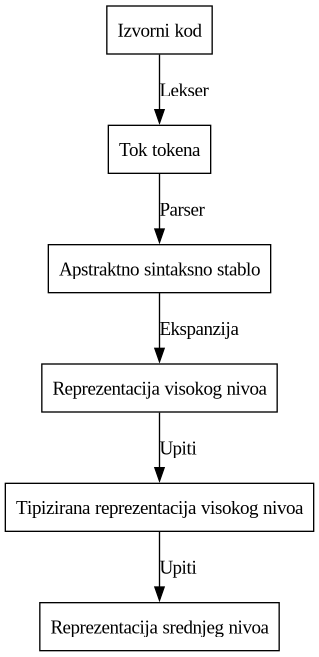
\includegraphics[width=2.5in, height=4.5in]{compilation.png}
\end{center}
\caption{Proces kompajliranja u prednjem kraju rustc-a}
\label{lst:compiler}
\end{listing}

\subsection{Tok tokena}

Uobičajno je da se lekseri programskih jezika implementiraju kao konačni automat uz pomoć alata kao što je
\verb|Flex|. Ipak, u jeziku Rust lekser je implementiran ručno. Ovo omogućava finu granularnost i visoku 
kontrolu nad procesom tokenizacije. Sa obzirom da je cilj Rust-a transparentne i korisne poruke o 
grešci, ovo je vrlo promišljena implementaciona odluka.
Kompajler poseduje naizgled dva leksera. Lekser niskog nivoa je \verb|rustc_lexer|, a lekser visokog nivoa je \verb|rustc_parse::lexer|. 
Obe implementacije su važne jer \verb|rusc_parse::lexer| koristi \verb|rustc_lexer| tokom kompajliranja.

\subsubsection{rustc\_lexer}

\verb|rustc_lexer| je lekser niskog nivoa koji poseduje sve osnovne
funkcionalnosti potrebne prilikom prikupljanja leksema.
Glavna funkcija iz ovog modula jeste \verb|tokenize| koja na osnovu celokupnog teksta 
izvornog koda dobavlja skup tokena tj. leksema \ref{lst:tokenize}.

\begin{listing}[H]
\begin{minted}{rust}
/// Creates an iterator that produces tokens from the input string.
pub fn tokenize(input: &str) -> impl Iterator<Item = Token> + '_ {
    let mut cursor = Cursor::new(input);
    std::iter::from_fn(move || {
        let token = cursor.advance_token();
        if token.kind != TokenKind::Eof { Some(token) } else { None }
    })
}
\end{minted}
\caption{Ulazna funkcija leksera}
\label{lst:tokenize}
\end{listing}

\newpage
Implementacija je bazirana na kursoru i unutar te strukture se nalazi celokupna logika leksera. 
Kursor je realizovan pomoću Rust-ovog iteratora i na osnovu njega prati trenutnu poziciju 
unutar izvornog koda. Veoma je bitna mogućnost gledanja ispred (\verb|look-ahead|) koja omogućava 
izvršavanje u jednom prolasku.
Kloniranje iteratora je jeftina operacija jer se svodi na kopiranje trenutne adresa.

\begin{listing}[H]
\begin{minted}{rust}
    /// Peeks the first symbol from the input stream without consuming it.
    pub fn first(&self) -> char {
        // `.next()` optimizes better than `.nth(0)`
        self.chars.clone().next().unwrap_or(EOF_CHAR)
    }

    /// Peeks the second symbol from the input stream without consuming it.
    pub(crate) fn second(&self) -> char {
        // `.next()` optimizes better than `.nth(1)`
        let mut iter = self.chars.clone();
        iter.next();
        iter.next().unwrap_or(EOF_CHAR)
    }

    /// Peeks the third symbol from the input stream without consuming it.
    pub fn third(&self) -> char {
        // `.next()` optimizes better than `.nth(1)`
        let mut iter = self.chars.clone();
        iter.next();
        iter.next();
        iter.next().unwrap_or(EOF_CHAR)
    }
\end{minted}
\caption{"Look-ahead" mehanizam}
\end{listing}
\verb|Token| sadrži samo informaciju o tipu token-a i njegovu dužinu ali ne i 
sam podatak.

\begin{listing}[H]
\begin{minted}{rust}
#[derive(Debug)]
pub struct Token {
    pub kind: TokenKind,
    pub len: u32,
}   
\end{minted}
\caption{Definicija "Token" strukture}
\end{listing}

\newpage
\subsubsection{rustc\_parse::lexer}

Lekser višeg nivoa \verb|rustc_parse::lexer| koristi \verb|rustc_lexer| prilikom izvršavanja sopstvenih
operacija. Bitna razlika je to što se sadržaj token analizira i postavlja u kontekst.
Lekser višeg nivoa koristi kursor svog prethodnika za dobavljanje leksema kroz strukturu \verb|StringReader|. 

\begin{listing}[H]
\begin{minted}{rust}
    struct StringReader<'psess, 'src> {
        psess: &'psess ParseSess,
        start_pos: BytePos,
        pos: BytePos,
        src: &'src str,
        cursor: Cursor<'src>,
        override_span: Option<Span>,
        nbsp_is_whitespace: bool,
        last_lifetime: Option<Span>,
    }
\end{minted}
\caption{Definicija "StringReader" strukture}
\end{listing}
\verb|StringReader| prati trenutnu poziciju unutar izvornog koda, a kursor 
dobavlja token koji ima odredjenu dužinu. Sadržaj tokena je niz karaktera sa početkom u \verb|pos|,
dužine od \verb|token.len|. 

Prolaskom kroz izvorni kod izvršavaju se sledeće akcije:
\begin{enumerate}
    \item Interniranje 
    \item Tokeni iz \verb|rustc_lexer| se mapiraju na tokene iz \verb|rustc_ast|
    \item Rezulucija zagrada svih tipova.
    \item Problemi i preporuke generišu dijagnostiku 
\end{enumerate}

Interniranje je proces u kome se stringovi pretvaraju internirane simbole. Na ovaj način
se čuva samo jedna nepromenljiva kopija sadržaja tokena. Tabela simbola je struktura podataka
koja čuva i održava O(1) pristup bilo kom simbolu.  Tabela simbola je implementirana pomoću \verb|IndexSet|
strukture. Ne internira se svaki token, već samo tokeni koji imaju varijabilnu dužinu.
\todo{Interniranje u pozadini koristi SpanData strukturu, u zavisnosti od specifičnih okolnosti
može koristiti manje ili veće Span-ove. Bitno je, ali nisam siguran da li zalaziti toliko u samu implementaciju.}

Mapiranje tokena iz leksera u tip tokena iz apstraktnog sintaksnog stabla je trivialno.
Za proste tipove vrši se jedan na jedan konverzija.

\begin{listing}[H]
\begin{minted}{rust}
    rustc_lexer::TokenKind::Semi => token::Semi,
    rustc_lexer::TokenKind::Comma => token::Comma,
    rustc_lexer::TokenKind::Dot => token::Dot,
\end{minted}
\caption{Prevodjenje tokena iz leksera u AST tokene}
\end{listing}
Za tipove koji imaju sadržaj u vidu nizova karaktera, sadržaj se internira i prenosi 
u novi token putem simbola \ref{lst:intern}. Derivati apstraktnog sintaksnog stabla se često koriste prilikom kompajliranja i zbog toga 
stablo mora biti memorijski optimizovano.

\begin{listing}[H]
\begin{minted}{rust}
    let ident = Symbol::intern(lifetime_name);
    token::Lifetime(ident, IdentIsRaw::No)
\end{minted}
\caption{Interniranje literala}
\label{lst:intern}
\end{listing}
Tok tokena je skup stabala tokena od kojih je svako stablo sačinjeno od skupa tokena.  
Rezolucija zagrada je proces unutar kog se validira da li je svaka zagrada pravilno zatvorena.
Rezolucija zagrada se dešava u samom vrhu procesa \verb|rustc_parser::lexer|-a 
za vreme kreiranja toka tokena. U kontekstu kompajlera zagrade se nazivaju delimiteri. 
Svaki otvoreni tip delimitera mora biti zatvoren delimiterom istog tipa koji je zatvoren.
Na primer, vitičasta zagrada je tip delimitera koja može biti otvoren (\{) ili zatvoren (\}) tj.
svaka otvorena vitičasta zagrada mora biti zatvorena zatvorenom vitičastom zagradom.

\begin{listing}[H]
\begin{minted}{rust}
fn lex_token_trees(
    &mut self,
    is_delimited: bool,
) -> (Spacing, TokenStream, Result<(), Vec<PErr<'psess>>>) {
    // Move past the opening delimiter.
    let (_, open_spacing) = self.bump(false);
    let mut buf = Vec::new();
    loop {
        match self.token.kind {
            token::OpenDelim(delim) => buf.push(match self
            .lex_token_tree_open_delim(delim) {
                Ok(val) => val,
                Err(errs) => return (open_spacing, 
                TokenStream::new(buf), Err(errs)),
            }),
            token::CloseDelim(delim) => {
                return (
                    open_spacing,
                    TokenStream::new(buf),
                    if is_delimited { 
                        Ok(()) 
                    } else { Err(vec![self.close_delim_err(delim)]) },
                );
            }
            token::Eof => {
                return (
                    open_spacing,
                    TokenStream::new(buf),
                    if is_delimited { Err(vec![self.eof_err()]) } 
                    else { Ok(()) },
                );
            }
            _ => {
                // Get the next normal token.
                let (this_tok, this_spacing) = self.bump(true);
                buf.push(TokenTree::Token(this_tok, this_spacing));
    } } } }
\end{minted}
\caption{Generisanje stabla tokena}
\end{listing}

\newpage

Primećuje se da u slučaju da kada delimiter ne postoji, dodavanje tokena u tok tokena 
je sekvencijalno i ne zahteva nikakvu kompleksnu logiku. Promenljiva \verb|is_delimited|
označava da li trenutna sekvenca tokena pripada nekom paru delimitera. U slučaju da 
se naidje na zatvoren tip delimitera bez da je prethodno postojao otvoren, vraća se greška
u vidu dijagnostike. U sličnom kontekstu, nailazak na token kraj-a fajla bez da je svaka 
zagrada zatvorena je greška. 
Nailaskom na \verb|token::Eof| ili \verb|token::CloseDelim| se završava prikupljanje toka tokena.
Ovo su veoma korisni granični slučajevi koji omogućavaju rekurziju. 

Obrada otvorenog tipa delimitera u pozadini poziva funkciju \verb|lex_token_trees| koji obradjuje
stablo tokena (deo toka tokena) izmedju novog para zagrada.
\begin{listing}[H]
\begin{minted}{rust}
    fn lex_token_tree_open_delim(
        &mut self,
        open_delim: Delimiter,
    ) -> Result<TokenTree, Vec<PErr<'psess>>> {
        // The span for beginning of the delimited section.
        let pre_span = self.token.span;

        self.diag_info.open_braces.push((open_delim, self.token.span));

        // Lex the token trees within the delimiters.
        // We stop at any delimiter so we can try to recover if the user
        // uses an incorrect delimiter.
        let (open_spacing, tts, res) = self
                            .lex_token_trees(/* is_delimited */ true);
        if let Err(errs) = res {
            return Err(self.unclosed_delim_err(tts, errs));
        }

        // Expand to cover the entire delimited token tree.
        let delim_span = DelimSpan::from_pair(pre_span, self.token.span);
        let sm = self.string_reader.psess.source_map();

        let close_spacing = match self.token.kind {
        .
        .
        .
\end{minted}
\caption{Parsiranje stabla tokena}
\end{listing}

Neobradjene zagrade se čuvaju u strukturi \verb|TokenTreeDiagInfo| u polju \verb|open_braces|.
Utvrdjeno je da će po uspešnom završetku izvršavanja funkcije \verb|lex_token_trees| 
trenutni token biti pozicioniran na zatvoreni tip delimiter-a. To omogućava validaciju 
pravilnog završetka zagrada.

\newpage
\subsection{Apstraktno Sintaksno Stablo}

Parser jezika Rust uz pomoć toka tokena iz leksera generiše apstraktno sintaksno stablo (AST). 
Prilikom poziva parsiranja, jedini fajl koji se odmah procesira jeste glavni \verb|main| fajl, potpuno stablo
nastaje putem ekspanzije i rezolucije imena.
Algoritam \verb|recursive-descent| se koristi tokom procesa parsiranja. Ovo je jedna od najjednostavnijih
tehnika parsiranja koja se koristi u praksi. Ovakvi parseri se takodje nazivaju \verb|top-down| parseri 
jer konstruišu stablo od gore ka dole \cite{parsing}. 

Parser koristi prethodno pomenuti tok tokena da bi kreirao kursor nad stablom tokena \verb|TokenTreeCursor|.
\verb|TokenStream| poseduje implementaciju \verb|into_tree| koji transformiše tip dobijen iz leksera
u tip pogodan parseru.

\begin{listing}[H]
\begin{minted}{rust}
pub fn into_trees(self) -> TokenTreeCursor {
    TokenTreeCursor::new(self)
}

impl TokenTreeCursor {
    fn new(stream: TokenStream) -> Self {
        TokenTreeCursor { stream, index: 0 }
    }
    ...
}
\end{minted}
\caption{Konverzija iz "TokenStream" u "TokenTreeCursor"}
\end{listing}
Jednostavnije je iterirati kroz stabla tokena sekvencijalno u odnosu na strukturu koja liči na kanape.

Za razliku od leksera, parser poseduje konstrukte koji su dosta složeniji od jednog tokena, kao što su 
strukture, enumeracije i slično (reč-rečenica poredjenje). Izvorni čvor \verb|AST|-a je \verb|Crate|.

\begin{listing}[H]
\begin{minted}{rust}
#[derive(Clone, Encodable, Decodable, Debug)]
pub struct Crate {
    pub attrs: AttrVec,
    pub items: ThinVec<P<Item>>,
    pub spans: ModSpans,
    pub id: NodeId,
    pub is_placeholder: bool,
}
\end{minted}
\caption{Definicija "Crate" strukture}
\end{listing}

\newpage

Najbitnija polja su atributi (\verb|attrs|) i stavke (\verb|items|). Atributi mogu biti spoljašnji ili unutrašnji.
Koriste se da bi korisnik pružio dodatne instrukcije kompajleru. 
Dodatne instrukcije mogu biti trivijalne poput dozvoljavanja
nekorišćenog koda, ali mogu biti i kompleksnije u vidu implementacije osobina 
(\verb|trait|). Osobina je funkcionalnost veoma slična interfejsu u drugim jezicima. 




Stavke su grupacije tokena iz leksera koje tako grupisane imaju semantiku. Iz perspektive koda 
veoma se malo razlikuje od samog \verb|Crate|-a. Svaka stavka poseduje identifikator \verb|NodeId| 
koji predstavlja sekvencijalni broj stavke unutar \verb|Crate|-a. Ovo znači da ukoliko se usred stabla 
obriše ili izgeneriše nova stavka, svaki čvor nakon tog dela stabla mora ponovo da izgeneriše svoj redni broj.
Samim time apstraktno sintaksno stablo nije korisno prilikom inkrementalne kompilacije jer su identifikatori
volotilni. Svaka stavka takodje sadrži \verb|Span|. Ovo je tip koji odredjuje početnu i krajnju poziciju 
stavke unutar izvornog koda. U odnosu na vrednost tipa \verb|kind|, stavke mogu ili ne mogu da poseduju atribute. 

\begin{listing}[H]
\begin{minted}{rust}
#[derive(Clone, Encodable, Decodable, Debug)]
pub struct Item<K = ItemKind> {
    pub attrs: AttrVec,
    pub id: NodeId,
    pub span: Span,
    pub vis: Visibility,
    pub ident: Ident,
    pub kind: K,
    pub tokens: Option<LazyAttrTokenStream>,
}
\end{minted}
\caption{Definicija "Item" strukture}
\end{listing}

\begin{listing}[H]
\begin{minted}{rust}
pub fn parse_crate_mod(&mut self) -> PResult<'a, ast::Crate> {
    let (attrs, items, spans) = self.parse_mod(&token::Eof)?;
    Ok(ast::Crate { attrs, items, spans, 
       id: DUMMY_NODE_ID, is_placeholder: false })
}
\end{minted}
\caption{Ulazna funkcija parsera}
\end{listing}


Rezolucija imena je jedan od delova formiranja apstraktnog sintaksnog stabla.
U programima se referenciraju funkcije, varijable i tipovi na osnovu imena. Ova imena nisu uvek jedinstvena.

\begin{listing}[H]
\begin{minted}{rust}
type a = u32;
let a: a = 1;
let b: a = 5; 
\end{minted}
\caption{Rezolucija imena}
\label{lst:resolution}
\end{listing}

Kako znamo, u izvornom kodu \ref{lst:resolution}, da li je u liniji 3 "a" tip ili vrednost 1?
Ovakvi konflikti se rešavaju prilikom rezolucije imena. U datom slučaju imena tipova i promenljivih se nalaze 
u različitim imenskim prostorima (\verb|namespaces|) i zbog toga mogu da koegzistiraju.
Rezolucija imena se izvodi iz dva faze. Prva faza se dešava za vreme ekspanzije (više o tome u daljem tekstu) 
gde se obradjuju samo \verb|import|-i. Druga faza se dešava nakon ekspanzije gde se obradjuje celokupno 
sintaksno stablo počevši od vrha pa na dole. 

Imena su validna u različitim delovima izvornog koda. Da bi se 
vreme života (\verb|scope|) nekog imena proverilo uvodi se koncept rebara (\verb|rib|). Svaki put kada se 
set vidljivih imena potencijalno menja novo rebro se gura na stek. Primeri situacija u kojima se dodaje 
novo rebro:
\begin{enumerate}
    \item Očigledna mesta kao što su vitičaste zagrade, funkcije, moduli.
    \item Prilikom poziva \verb|let| jer se ime može redefinisati (\verb|shadowing|).
    \item Početak proširenja makroa. 
\end{enumerate}
Potraga za imenom se izvodi od najdubljeg rebra (vrh steka) ka najplićem. 
Redosled je veoma bitan zato što se ovakvom pretragom izbegava greška 
ukoliko je neko ime redefinisano.

\begin{listing}[H]
\begin{minted}{rust}
let a: u32 = 1;
let a: i32 = -1;
\end{minted}
\caption{"Shadowing"}
\label{lst:shadowing}
\end{listing}
\newpage

Jezici kao što je C pored kompajlera sadrže pre-procesor koji prikuplja izvorni kod. 
Prilikom prikupljanja izvornog koda skraćenice (makroi) se proširuju na izraze programskog jezika. 
Rust se odlikuje veoma moćnim makroima ali ne poseduje pre-procesor. Transformacija skraćenica se vrši 
putem ekspanzije.  Ekspanzija je proces tokom kog se dopunjuje apstraktno sintaksno stablo
proširivnajem makroa i umetanjem modula (\verb|inlining|). Prilikom parsiranja umesto 
modula i makroa se postavljaju AST fragmenti. Ovi fragmenti su početne tačke algoritma ekspanzije.
Kreira se red čekanja neproširenih makroa. Jedan po jedan se uzimaju iz reda čekanja, vriši se rezolucija imena,
proširuju se i integrišu nazad u stablo. U slučaju da se nema napretka (loše napisan kod), vraća se greška.

Pre nego što počne prelazak u sledeći posredni oblik AST stablo se validira. 
Tokom prolaska se proverava da li je stablo sintaktički validno, bez ikakvih kompleksnih analiza,
rezolucije imena ili provera tipova. Ovo nije moguće učiniti prilikom parsiranja jer makro atributi 
omogućavaju odredjene delove netačne sintakse kao što je funkcija bez tela van definicije osobine (\verb|trait|) \ref{lst:validate}.

\begin{listing}[H]
\begin{minted}{rust}
#[attribute]
mod foo {
    fn missing_body();
}
\end{minted}
\caption{"Netačna sintaksa pre ekspanzije"}
\label{lst:validate}
\end{listing}
\todo{Mogu da napišem makro koji bi proširio telo funkcije, da li da dodam?}

Apstraktno sintaksno stablo pre i posle ekspanzije nekog \verb|Crate|-a se može analizirati pomoću 
nestabilnih \verb|-Z| zastavica \ref{lst:rustc_ast}.

\todo{Sam prikaz AST-a nije naročito interesantan, a čak i za najjednostavnije programe a + b ume da bude 
pozamašne dužine}

\begin{listing}[H]
\begin{minted}{bash}
cargo rustc -- -Z unpretty=ast
cargo rustc -- -Z unpretty=ast,expanded
\end{minted}
\caption{"Prikaz apstraktnog sintaksnog stabla"}
\label{lst:rustc_ast}
\end{listing}

\newpage
\subsection{Posredna Reprezentacija Visokog Nivoa - HIR (High-Level Intermediate Representation)}

\todo{try mark green algoritam}

Posredna reprezentacija visokog nivoa je primarna posredna reprezentacija koja se koristi 
u većinskom delu \verb|rustc| kompajlera. HIR je posledica snižavanja (\verb|lowering|). 
Tokom procesa snižavanja, neke forme izražavanja bivaju pojednostavljene (\verb|desugared|):
\begin{enumerate}
    \item Zagrade se uklanjaju jer struktura stabla eksplicitno odredjuje redosled operacija.
    \item for petlje su konvertovane u while(let) petlje \ref{lst:hir_iter}.
    \item if let se konvertuje u match.
    \item impl u parametrima funkcije se konvertuje u generičke argumente.
\end{enumerate}

\begin{listing}[H]
\begin{minted}{rust}
// Pre
for elem in vec {
    process(elem);
}

// Posle
let mut iterator = vec.into_iter();
while let Some(elem) = iterator.next() {
    process(elem);
}
\end{minted}
\caption{"for" petlja pre i posle pojednostavljenja}
\label{lst:hir_iter}
\end{listing}

HIR prikazuje samo trenutno stanje \verb|Crate|-a.
Samim time sadrži samo funkcije drugih modula koje su implicitno ili eskplicitno korišćene 
od strane glavnog modula, sve ostalo će biti ignorisano.

Glavni čvor HIR-a se isto kao i kod AST-a naziva \verb|Crate| ali sadrži drugačije podatke,
veliki broj mapa koje služe da omoguće lakši pristup sadržaju.

HIR poseduje proširen spektar identifikatora:
\begin{enumerate}
    \item DefId - referencira definiciju unutar bilo kog \verb|Crate|-a.
    \item LocalDefId - referencira definiciju unutar trenutno kompajliranog \verb|Crate|-a.
    \item HirId - referencira bilo koji čvor u HIR-u.
\end{enumerate}

Većinu vremena HIR-u se pristupa pomoću HIR mape. HIR mapa sadrži brojne metode 
koje na osnovu različitih tipova identifikatora dobavljaju podatke.
\todo{Nisam zadovoljan ovim delom, potrebno je ako ništa objasniti zašto su ovi identifikatori korisni
u vidu inkrementalne kompilacije}

\newpage
\subsection{Tipizirana Posredna Reprezentacija Visokog Nivoa - THIR (Typed High-Level Intermediate Representation)}

Tipizirani HIR je posredna reprezentacija izvornog koda koja se generiše tokom provere tipova, jer je potrebno
da su tipovi unutar celog stabla popunjeni. THIR sadrži samo tela (obično tela funkcija) tj. izvršni kod.
Posledica ovoga jeste nedostatak reprezentacija struktura i osobina. 
Rust ima odliku da ukoliko se koristi neki vid provere šablona (\verb|pattern matching|) svaki tip unutar 
šablona mora biti pokriven \ref{lst:pattern_matching}. Proveru da li je svaki tip obradjen izvršava THIR.

\begin{listing}[H]
\begin{minted}{rust}
pub enum IpAddrKind {
    V4,
    V6,
}

fn main() {
    let x = IpAddrKind::V4;
    match x {
        IpAddrKind::V4 => println!("Ovo je IPv4 adresa."), 
        // Pokriven IpAddrKind::V4
        IpAddrKind::V6 => println!("Ovo je IPv6 adresa.") 
        // Pokriven IpAddrKind::V6
        // Da je postojao IpAddrKind::V7 Rust bi zahtevao 
        // da i ta varijanta bude obradjena.
    }
}
\end{minted}
\caption{Provera šablona}
\label{lst:pattern_matching}
\end{listing}

Za razliku od HIR-a koji je perzistiran tokom celokupnog izvršavanja kompajlera, THIR se odbacuje momenta
kada više nema upotrebnu vrednost. Pored toga što su svi tipovi čvorova prisutni, THIR se odlukuje dodatnim 
pojednostavljivanjem koda:
\begin{enumerate}
    \item Automatska referenciranja i dereferenciranja su eksplicitna.
    \item Pozivi metoda i opterećeni operatori su konvertovani u obične pozive funkcija. 
    \item Obim životnog veka je eksplicitan.
\end{enumerate}
% Izrazi, iskazi i \verb|match| ruke se čuvaju zasebno. 

Pojednostavljenje čini THIR podobnim za proveru nebezbednog koda jer fundamentalno poseduje manje opcija, 
nebezbedni pozivi metoda i nebezbedni pozivi funkcija imaju identičnu reprezentaciju. Ova provera 
iskazuje grešku ako je nebezbedna operacija korišćena van \verb|unsafe| opsega.

\todo{THIR je kratak sam po sebi ali moguće je detaljnije obraditi pattern matching}

\newpage
\subsection{Posredna Reprezentacija Srednjeg Nivoa - MIR (Mid-Level Intermediate Representation)}

Prvobitno koncept \verb|MIR|-a nije postojao. HIR se transformisao u LLVM reprezentaciju gde 
vršila optimizacija. Glavni povod za uvod reprezentacije srednjeg nivoa 
jeste inkrementalna kompilacija i MIR je struktuiran tako da ga je lako sačuvati i učitati, iako su se delovi
koda promenili tokom vremena.

U HIR-u optimizacija \verb|for| petlje je svedena na \verb|while(let)| u MIR-u se prevodi na \verb|loop match| 
primitivu \ref{lst:mir_for_1}.  Pozivi metoda su prevedeni u pozive funkcija još u THIR-u.

\begin{listing}[H]
\begin{minted}{rust}
let mut iterator = IntoIterator::into_iter(vec);
loop {
    match Iterator::next(&mut iterator){
        Some(elem) => process(elem),
        None => break,
    }
}
\end{minted}
\caption{"while let" posle pojednostavljenja}
\label{lst:mir_for_1}
\end{listing}

Reprezentacija srednjeg nivoa dozvoljava za još jedan vid optimizacije na nivou frontenda pojednostavljivanjem
sintakse na primitive koje nisu dostupne u regularnom jeziku.

\begin{listing}[H]
\begin{minted}{rust}
let mut iterator = IntoIterator::into_iter(vec);

loop:
    match Iterator::next(&mut iterator) {
        Some(elem) => { process(elem); goto loop; }
        None => { goto break; }
    }

break:
\end{minted}
\caption{"while let" posle pojednostavljenja}
\label{lst:mir_for_2}
\end{listing}

Izraz \verb|goto| je u inženjerskoj zajednici gledan sa visine jer kontrola toka nakon odredjene kompleksnosti
postaje nerazumljiva. Rust iz istog razloga ne dozvoljava upotrebu ove ključne reči, ali u MIR-u svodi 
petlju na najjednostavniji oblik \ref{lst:mir_for_2}.

\newpage
U isečku koda \ref{lst:mir_for_2}, jedina kompleksnija sintaktička celina je \verb|match|. U samom jeziku 
grupisanje provere i pristup podatku je smisleno ali u MIR-u se odvaja na dve celine \ref{lst:mir_for_3}.

\begin{listing}[H]
\begin{minted}{rust}
loop:
    let tmp = Iterator::next(&mut iterator);
    
    switch tmp {
        Some => {
            let elem = (tmp as Some).0;
            process(elem);
            goto loop;
        }
        None => {
            goto break;
        }
    }
    
break:
    ....
\end{minted}
\caption{"while let" posle pojednostavljenja}
\label{lst:mir_for_3}
\end{listing}

Naime ovako sveden kod nikada nije tekstualnom obliku. MIR je graf kontrole toka koji se može predstaviti
uz pomoć \verb|graphviz|-a \ref{lst:mir_print}. Filter mora biti zadatat prilikom poziva ove komande. 
Za prikaz celokupnog izlaza koristi se \verb|all| filter, dok ako je neka pojedinačna funkcija od interesovanja
njeno ime (mnogo češće slučaj).

\begin{listing}[H]
\begin{minted}{bash}
cargo rustc -- -Z dump-mir=[filter] -Z dump-mir-graphviz
\end{minted}
\caption{Ispis i prikaz MIR-a}
\label{lst:mir_print}
\end{listing}

\todo{MIR je opsežan, ne izgleda kao u primerima (umereni nivo obfuskacije). Ovde ima još značajno puno sadržaja koji nije opisan.}

\newpage
\section{Zaključak}

\newpage
\section{Literatura}

\begin{thebibliography}
    \raggedright
\bibitem{msrc} 
    MSRC, “A proactive approach to more secure code | MSRC Blog | 
    Microsoft Security Response Center,” Microsoft.com, Jul. 16, 2019. 
    \url{https://msrc.microsoft.com/blog/2019/07/a-proactive-approach-to-more-secure-code/} 
    (pristupljeno Sep. 08, 2024).

    \bibitem{parsing} 
    “Parsing” Rochester.edu, 2024.
    \url{https://www.cs.rochester.edu/u/nelson/courses/csc_173/grammars/parsing.html#:~:text=Recursive%2Ddescent%20parsing%20is%20one,non%2Dterminal%20with%20a%20procedure} 
    (pristupljeno Sep. 21, 2024).

    \bibitem{dragonbook} 
    A. V. Aho, M. S. Lam, R. Sethi, and J. D. Ullman, \emph{Compilers: Principles, Techniques, and Tools}, 2nd ed. Boston, MA, USA: Addison-Wesley, 2006.

    \bibitem{rust-guide} 
    “Getting Started - Rust Compiler Development Guide,” Rust-lang.org, 2024. 
    \url{https://rustc-dev-guide.rust-lang.org/getting-started.html} (pristupljeno Sep. 28, 2024).

    \bibitem{rust-reference}
    “Introduction - The Rust Reference,” Rust-lang.org, 2015. 
    \url{https://doc.rust-lang.org/reference/introduction.html} (pristupljeno Sep. 29, 2024).
    
    \bibitem{rustonomicon}
    “Meet Safe and Unsafe - The Rustonomicon,” Rust-lang.org, 2024. 
    \url{https://doc.rust-lang.org/nomicon/meet-safe-and-unsafe.html} (pristupljeno Sep. 29, 2024).

    \bibitem{editions}
    “What are editions? - The Rust Edition Guide,” Rust-lang.org, 2024.
    \url{https://doc.rust-lang.org/edition-guide/editions/} (pristupljeno Okt. 03, 2024).

    \bibitem{unstable}
    “The Unstable Book - The Rust Unstable Book,” Rust-lang.org, 2024. 
    \url{https://doc.rust-lang.org/unstable-book/index.html} (pristupljeno Okt. 06, 2024).

    \bibitem{unstable-flagsunstable}
    Li, Chenghao, et al. “Demystifying Compiler Unstable Feature Usage and Impacts in the Rust Ecosystem.” 26 Oct. 2023. arXiv, Accessed 6 Oct. 2024. 

    \bibitem{rust-language}
    Bugden W, Alahmar A. Rust: The programming language for safety and performance. arXiv preprint arXiv:2206.05503. 2022 Jun 11.

    \bibitem{supply-chain}
    P. Mainardi, “The Rising Threat of Software Supply Chain Attacks: Managing Dependencies of Open Source projects,” Linuxfoundation.eu, Aug. 15, 2023.
    \url{https://linuxfoundation.eu/newsroom/the-rising-threat-of-software-supply-chain-attacks-managing-dependencies-of-open-source-projects} (pristupljeno Okt. 20, 2024).
‌
\end{thebibliography}

\newpage
\section{Dodatak 1}

\newpage
\section{Podaci o kandidatu}


Kandidat Aleksa Bajat rođen je 2001. godine u Novom Sadu. Završio je prirodno-matematički smer na engleskom jeziku 
u gimnaziji "Jovan Jovanović Zmaj" 2019. godine. Tokom sve četiri godine gimnazije uspešno je pohadjao 
"Centar za mlade talente" kompanije Schneider Electric.  Godine 2019. upisao je Fakultet 
Tehničkih Nauka u Novom Sadu, gde je ispunio sve obaveze i položio sve ispite predviđene 
studijskim programom sa prosečnom ocenom 9.03.

\end{document}
